%%%%%%%%%%%%%%%%%%%%%%%%%%%%%%%%%%%%%%%%%%%%%%%%%%%%%%%%%%%%%%%%%%%%%%%%%%%%%%%%%%%%%%%%%%%%%%%%%%%
%%%%%%%%%%%%%%%%%%%%%%%%%%%%%%%%%%%%%%%%%%%%%%%%%%%%%%%%%%%%%%%%%%%%%%%%%%%%%%%%%%%%%%%%%%%%%%%%%%%
\subsection{Tag Manager}\label{tag_manager}
% TODO: schéma résumant l'utilisation : clap -> soit sockets, soit modif fichiers avec lib
% Schéma vertical avec flèches
%%%%%%%%%%%%%%%%%%%%%%%%%%%%%%%%%%%%%%%%%%%%%%%%%%%%%%%%%%%%%%%%%%%%%%%%%%%%%%%%%%%%%%%%%%%%%%%%%%%
%%%%%%%%%%%%%%%%%%%%%%%%%%%%%%%%%%%%%%%%%%%%%%%%%%%%%%%%%%%%%%%%%%%%%%%%%%%%%%%%%%%%%%%%%%%%%%%%%%%
\subsubsection{Description du programme et du code}\label{tag_manager_description}
La première réalisation de ce projet est un outil en ligne de commande, écrit en Rust, permettant 
de facilement lister, ajouter et supprimer des tags à des fichiers et dossiers (avec une option 
récursive pour les dossiers) et d'exécuter des requêtes vers le serveur (Tag Engine, sous-section 
\ref{tag_engine_realisation}) pour lister 
les tags existants, renommer un tag et demander la liste des fichiers correspondant à des tags 
donnés. Cet outil dépend de deux \textit{crates} disponibles sur \href{https://crates.io}{crates.io} 
: clap \cite{ref22} et xattr \cite{ref23}.
\subparagraph{clap}
(Command Line Argument Parser for Rust) est une 
librairie pour parser les arguments d'un programme en ligne de commande. Elle s'occupe d'analyser 
et de valider les arguments fournis par l'utilisateur. Elle dispose de plusieurs syntaxes pour 
définir les arguments des commandes de notre programme. Sur le dépôt github de clap, dans le 
dossier \textit{examples}, plusieurs exemples d'utilisation sont fournis. Pour illustrer son 
utilisation, le listing \ref{tag_manager_clap} reprend l'exemple \mintinline{text}{01a_quick_example.rs} 
avec la plupart des commentaires tronqués et des adaptations de mise en page. Des lignes 2 à 13, 
les arguments attendus et les informations sur l'application sont définis avec entre autres la 
version du programme, le nom de l'auteur, etc. Dans cet exemple, les arguments sont définis à 
partir d'une chaîne de caractères respectant un format bien spécifique. clap génère automatiquement 
une aide au programme à partir des arguments définis s'il est lancé sans aucun des arguments attendus.
À partir de la ligne 15, les arguments reçus sont utilisés. La méthode \mintinline{rust}{value_of()} 
retourne la valeur d'un argument présent à l'exécution. Il est donc aisé d'utiliser les arguments 
donnés en tant que variables du programme. clap donne également la possibilité de regrouper les 
arguments. Un seul argument d'un groupe peut être présent à l'exécution, ce qui évite de nombreuses 
conditions de détection des arguments.
\subparagraph{xattr}
est une \acrshort{api} 
en Rust pour récupérer, lister, ajouter/modifier et supprimer des \acrshort{xattr} accrochés à des 
fichiers avec Rust. C'est essentiellement un wrapper des \acrshort{syscall} en C fournis par Linux 
et d'autres \acrshort{os} pour manipuler les \acrshort{xattr}. À noter que les fonctions offertes ne 
suivent pas les liens symboliques (il est fait de même pour Tag Manager lui-même). Quatre fonctions 
sont disponibles : \mintinline{rust}{get()}, \mintinline{rust}{list()}, \mintinline{rust}{set()} 
et \mintinline{rust}{remove()}. Toutes attendent le nom du fichier et selon les cas le nom du 
\acrshort{xattr} ainsi que sa valeur.
\bigbreak
\begin{code}
    \begin{minted}[bgcolor=mygray,breaklines,breaksymbol=,linenos,frame=single,stepnumber=1,tabsize=2]{rust}
fn main() {
    let matches = App::new("MyApp")
        .version("1.0")
        .author("Kevin K. <kbknapp@gmail.com>")
        .about("Does awesome things")
        .args_from_usage(
            "-c, --config=[FILE] 'Sets a custom config file'
            <output> 'Sets an optional output file'
            -d... 'Turn debugging information on'")
        .subcommand(SubCommand::with_name("test")
            .about("does testing things")
            .arg_from_usage("-l, --list 'lists test values'"))
        .get_matches();

    if let Some(o) = matches.value_of("output") {
        println!("Value for output: {}", o);
    }
    if let Some(c) = matches.value_of("config") {
        println!("Value for config: {}", c);
    }

    match matches.occurrences_of("d") {
        0 => println!("Debug mode is off"),
        1 => println!("Debug mode is kind of on"),
        2 => println!("Debug mode is on"),
        3 | _ => println!("Don't be crazy"),
    }

    if let Some(matches) = matches.subcommand_matches("test") {
        if matches.is_present("list") {
            println!("Printing testing lists...");
        } else {
            println!("Not printing testing lists...");
        }
    }
}
    \end{minted}
    \caption{Exemple d'utilisation de clap (commentaires tronqués) - \cite{ref42}}
    \label{tag_manager_clap}
\end{code}
\bigbreak
Tag Manager est constitué de deux fichiers. Le premier, \mintinline{rust}{main.rs} contient les 
définitions et détections des arguments fournis par l'utilisateur avec clap (voir listing 
\ref{tag_manager_main_args}), les appels aux fonctions 
manipulant les \acrshort{xattr} des fichiers et la partie socket de connexion, requête et attente 
de réponse du serveur (Tag Engine, sous-section \ref{tag_engine_realisation}). Le deuxième fichier, 
\mintinline{rust}{lib.rs}, contient l'\acrshort{api} publique pour récupérer, attribuer, renommer 
et supprimer les tags pour un fichier donné et un module de test de ces fonctions. À noter que 
dans les \textit{output} du programme, il n'y a pas de distinction entre fichiers et répertoires.
À titre d'exemple, 
le listing \ref{tag_manager_del_tags} montre le code de la fonction \mintinline{rust}{del_tags()} 
qui supprime les tags donnés d'un fichier. Elle préserve les tags existants qui ne doivent pas être 
supprimés et supprime totalement le \acrshort{xattr} en cas de tableau de tags vide. L'usage 
des \mintinline{rust}{enum} \mintinline{rust}{Option} et \mintinline{rust}{Result} en association 
avec des \textit{pattern matching} sont utilisées dès que possible.
\bigbreak
\begin{code}
    \inputminted[bgcolor=mygray,breaklines,breaksymbol=,linenos,frame=single,stepnumber=1,
        tabsize=2,firstline=37,lastline=56]{rust}{../tag_manager/src/main.rs}
    \caption{Déclaration des arguments dans \mintinline{rust}{main.rs}}
    \label{tag_manager_main_args}
\end{code}
\bigbreak
\bigbreak
\begin{code}
    \inputminted[bgcolor=mygray,breaklines,breaksymbol=,linenos,frame=single,stepnumber=1,
        tabsize=2,firstline=52,lastline=79]{rust}{../tag_manager/src/lib.rs}
    \caption{Code de la fonction \mintinline{rust}{del_tags()} dans \mintinline{rust}{lib.rs}}
    \label{tag_manager_del_tags}
\end{code}
\bigbreak
La communication socket est réalisée grâce la librairie standard \mintinline{rust}{UnixStream}, 
équivalent aux sockets \mintinline{c}{AF_UNIX} en C (voir sous-section \ref{sockets_doc}). Le 
fichier adresse des sockets est par défaut écrit dans \mintinline{text}{/tmp/tag_engine}. Le format 
des requêtes respecte le petit protocole décrit dans la table \ref{tag_manager_sockets_protocol}.
La requête listant les fichiers selon une expression logique des tags accepte les opérateurs 
\mintinline{text}{AND} et \mintinline{text}{OR}, avec la précédance logique du premier sur le 
second (voir sous-section \ref{tag_engine_realisation} pour plus de détails). Les opérateurs et 
opérandes (les tags) doivent être espacés par un espace.
\begin{center}
    \begin{tabular}{|p{6cm}|c|p{6cm}|} \hline
        \textbf{Requête} & \textbf{Code} & \textbf{Exemple} \\ \hline
        Fichers et dossiers correspondant à une expression logique de tags & \mintinline{text}{0x0} & 
            \mintinline{text}{0x0 tag1 OR tag2 AND tag3} \\ \hline
        Liste des tags existants & \mintinline{text}{0x1} & \mintinline{text}{0x1} \\ \hline
        Renommage d'un tag & \mintinline{text}{0x2} & \mintinline{text}{0x2 old_name new_name} \\ \hline
    \end{tabular}
    \captionof{table}{Format du protocole des requêtes au serveur Tag Engine}
    \label{tag_manager_sockets_protocol}
\end{center}

%%%%%%%%%%%%%%%%%%%%%%%%%%%%%%%%%%%%%%%%%%%%%%%%%%%%%%%%%%%%%%%%%%%%%%%%%%%%%%%%%%%%%%%%%%%%%%%%%%%
%%%%%%%%%%%%%%%%%%%%%%%%%%%%%%%%%%%%%%%%%%%%%%%%%%%%%%%%%%%%%%%%%%%%%%%%%%%%%%%%%%%%%%%%%%%%%%%%%%%
\subsubsection{Utilisation du programme et exemples}
L'utilisation des différents arguments du programme est résumée dans la table \ref{tag_manager_usage}. 
Les arguments sont divisés en deux groupes, le premier pour manipuler directement les fichiers et 
leurs tags, le deuxième pour exécuter des requêtes au serveur Tag Engine. Pour le premier groupe, 
l'argument \mintinline{text}{-f} ou \mintinline{text}{--files} est obligatoire. Pour les opérations 
du deuxième groupe, il faut évidemment que le serveur Tag Engine soit lancé.
\begin{center}
    \begin{tabular}{|p{3.7cm}|p{2.3cm}|p{8.5cm}|} \hline
        \textbf{Opération} & \textbf{Arguments} & \textbf{Exemple} \\ \hline
        Afficher l'aide & \mintinline{text}{-h} & \mintinline{text}{tag_manager -h} \\ \hline
        Afficher les tags d'un ou plusieurs fichiers & 
            \mintinline{text}{-f} ou \mintinline{text}{--files} & 
            \mintinline{text}{tag_manager -f file1 file2} \\ \hline
        Afficher les tags d'un dossier récursivement & 
            \mintinline{text}{-r} ou \mintinline{text}{--recursive} & 
            \mintinline{text}{tag_manager -f myfolder -r} \\ \hline
        Attribuer des tags à un ou plusieurs fichiers & 
            \mintinline{text}{-s} ou \mintinline{text}{--set} & 
            \mintinline{text}{tag_manager -f file1 file2 -s bob fred} \\ \hline
        Supprimer des tags à un ou plusieurs fichiers & 
            \mintinline{text}{-d} ou \mintinline{text}{--del} & 
            \mintinline{text}{tag_manager -f file1 file2 -d bob fred} \\ \hline
        Lister les fichiers correspondants à une requête de tags & 
            \mintinline{text}{-q} ou \mintinline{text}{--query} & 
            \mintinline{text}{tag_manager -q bob AND fred} \\ \hline
        Lister les tags existants & 
            \mintinline{text}{-l} ou \mintinline{text}{--list} & 
            \mintinline{text}{tag_manager -l} \\ \hline
        Renommer un tag & 
            \mintinline{text}{-R} ou \mintinline{text}{--rename} & 
            \mintinline{text}{tag_manager -R old_name new_name} \\ \hline
    \end{tabular}
    \captionof{table}{Utilisation et arguments attendus par Tag Manager}
    \label{tag_manager_usage}
\end{center}
Le listing \ref{tag_manager_ex} illustre les usages et retours de Tag Manager. Le terminal se situe 
dans le répertoire \mintinline{text}{home} de l'utilisateur. Tout d'abord, Tag Manager est utilisé pour 
lister récursivement les tags des fichiers et sous-dossiers donnés, attribuer les tags \mintinline{text}{in_a} 
et \mintinline{text}{myfiles} à différents fichiers et dossiers, lister les tags existants et faire 
une requête sur les deux tags. L'arborescence utilisée pour l'exemple se situe dans le répertoire 
\mintinline{text}{home} de l'utilisateur et est constituée des quatre fichiers et deux répertoires suivants :
\dirtree{%
.1 a.
.2 a1.
.2 a2.
.2 b.
.3 b1.
.3 b2.
}
\bigbreak
\begin{code}
    \inputminted[bgcolor=mygray,breaklines,breaksymbol=,linenos,frame=single,stepnumber=1,
        tabsize=2]{bash}{text/tag_manager_ex.txt}
    \caption{Exemples d'utilisation de Tag Manager}
    \label{tag_manager_ex}
\end{code}
\bigbreak


%%%%%%%%%%%%%%%%%%%%%%%%%%%%%%%%%%%%%%%%%%%%%%%%%%%%%%%%%%%%%%%%%%%%%%%%%%%%%%%%%%%%%%%%%%%%%%%%%%%
%%%%%%%%%%%%%%%%%%%%%%%%%%%%%%%%%%%%%%%%%%%%%%%%%%%%%%%%%%%%%%%%%%%%%%%%%%%%%%%%%%%%%%%%%%%%%%%%%%%
\subsection{Tag Engine}\label{tag_engine_realisation}
%%%%%%%%%%%%%%%%%%%%%%%%%%%%%%%%%%%%%%%%%%%%%%%%%%%%%%%%%%%%%%%%%%%%%%%%%%%%%%%%%%%%%%%%%%%%%%%%%%%
%%%%%%%%%%%%%%%%%%%%%%%%%%%%%%%%%%%%%%%%%%%%%%%%%%%%%%%%%%%%%%%%%%%%%%%%%%%%%%%%%%%%%%%%%%%%%%%%%%%
\subsubsection{Description du programme et du code}
La deuxième réalisation de ce projet est un programme "indexant" (ne crée pas un index au sens 
strict du terme, voir explications plus loin) et surveillant une arborescence de 
répertoires, fichiers et tags associés. Ce programme fait également office de serveur pour les 
requêtes émises depuis Tag Manager. Il est divisé en plusieurs fichiers et modules :
% TODO: expliquer mutex + arc
\begin{itemize}
    \item \mintinline{rust}{graph.rs} : module relatif à la construction et 
        maintenance du graphe des tags, fichiers et répertoires (voir paragraphe \textbf{petgraph}).
    \item \mintinline{rust}{lib.rs} : regroupe les modules et contient la fonction 
        \mintinline{rust}{dispatcher()}, appelée lors d'un événement sur l'arborescence surveillée 
        (voir paragraphe \textbf{notify}).
    \item \mintinline{rust}{main.rs} : point d'entrée du programme, initialise les variables 
        partagées, le thread socket serveur et écoute indéfiniment sur les événements survenus 
        sur l'arborescence surveillée (voir paragraphe \textbf{Threads et \textit{channel}}).
    \item \mintinline{rust}{parse.rs} : module de conversion d'une expression infixe vers postfixe 
        (voir paragraphe \textbf{Analyse d'une expression logique}).
    \item \mintinline{rust}{server.rs} : module construisant le serveur socket et répondant 
        aux différentes requêtes émises depuis Tag Manager (voir paragraphe \textbf{Serveur sockets}).
\end{itemize}
% TODO: schéma résumant l'utilisation
Ce programme dépend de quatre \textit{crates}. Le premier est 
tag\_manager (la librairie des fonctions manipulant les \acrshort{xattr}, voir sous-section \ref{tag_manager}), 
réalisé au cours de ce projet. Les trois autres sont disponibles sur \href{https://crates.io}{crates.io}, 
il s'agit de walkdir \cite{ref43}, petgraph \cite{ref44} et notify \cite{ref45}.

% TODO: Utilisation de tag manager lib
% \subparagraph{tag\_manager}
% est repris ici pour deux de ses fonctions publiques : \mintinline{rust}{get_tags()} et 
% \mintinline{rust}{rename_tag()}. La première 

\subparagraph{walkdir}
est une librairie pour parcourir efficacement et de manière récursive une arborescence de fichiers.
Elle offre différentes structures, dont \mintinline{rust}{WalkDir} et \mintinline{rust}{DirEntry}. 
\mintinline{rust}{WalkDir} attend un chemin de répertoire et retourne un itérateur récursif sur 
chaque sous-répertoire et fichier contenu dans le répertoire de départ. Chaque entrée de cet 
itérateur est représenté par la structure \mintinline{rust}{DirEntry}, qui détient des méthodes 
pour obtenir des informations sur l'entrée (le chemin complet, les méta-données, si c'est un 
répertoire ou un fichier, son nom, etc.). Le listing \ref{walkdir_demo} illustre un exemple de 
parcours d'un répertoire. walkdir est utilisé pour réaliser le premier scan de l'arborescence 
fournie et constituer le graphe (voir listing \ref{tag_engine_graph_make_graph}).
\bigbreak
\begin{code}
    \begin{minted}[bgcolor=mygray,breaklines,breaksymbol=,linenos,frame=single,stepnumber=1,tabsize=2]{rust}
use walkdir::WalkDir;

fn main() {
    for entry in WalkDir::new("/home") {
        let entry = entry.unwrap();
        println!("{}", entry.path().display());
    }
}
    \end{minted}
    \caption{Parcours d'un répertoire avec walkdir}
    \label{walkdir_demo}
\end{code}
% \bigbreak

\subparagraph{petgraph}\label{tag_engine_petgraph}
est une librairie de représentation de graphes. Elle fournit différentes structures de données pour 
représenter un graphe et des modules de manipulation et parcours de graphes. Les structures de 
données sont au nombre de trois :
\begin{enumerate}
    \item \mintinline{rust}{Graph<N, E, Ty = Directed, Ix = DefaultIx>} : représente un graphe et 
        ses données sous forme de deux listes d'adjacence (deux \mintinline{rust}{Vec}, un pour les 
        noeuds et l'autre pour les arcs ou arêtes). Les noeuds sont de type générique \mintinline{rust}{N}, 
        les arcs ou arêtes de type générique \mintinline{rust}{E}, le graphe est par défaut orienté (type 
        \mintinline{rust}{Directed}) et le type pour l'index (l'identifiant numérique d'un noeud et 
        d'un arc ou arête dans les vecteurs respectifs, déterminant la taille maximale du graphe) 
        est par défaut \mintinline{rust}{u32} (ce qui autorise plus de quatre milliards de noeuds, 
        4'294'967'296 précisément).
    \item \mintinline{rust}{StableGraph<N, E, Ty = Directed, Ix = DefaultIx>} : semblable à 
        \mintinline{rust}{Graph}, avec une différence notable, elle garde les identifiants des noeuds et 
        arcs ou arêtes supprimés. Cette structure comporte également moins de méthodes.
    \item \mintinline{rust}{GraphMap<N, E, Ty>} : représente un graphe et ses données sous forme 
        d'une table associative, dont les clés sont les noeuds de type générique \mintinline{rust}{N}, 
        avec l'obligation pour ce type d'être conforme pour l'utilisation en tant que clé. Permet 
        de tester l'existence d'un noeud en temps constant avec la contrepartie de ne pas pouvoir 
        stocker plus qu'un noeud avec une même donnée.
\end{enumerate}
Avant de continuer les explications sur l'utilisation de petgraph, faisons un bref rappel de l'architecture 
choisie pour représenter l'arborescence des fichiers et tags à surveiller. Un noeud du graphe peut 
être soit un fichier, soit un répertoire, soit un tag. Le lien entre un répertoire et un sous-répertoire 
ou un fichier est symbolisé par un arc partant du répertoire en question. Le lien entre un tag et 
un répertoire ou un fichier est également un arc partant du tag en question. Un arc n'a pas de 
donnée à sauvegarder, il n'a donc pas de type effectif. Pour accélérer l'accès à un tag dans le 
graphe à partir de son nom, une \textit{hashmap} associant le nom du tag à son identifiant dans le graphe 
est maintenue.

La structure \mintinline{rust}{StableGraph} a été choisie en raison de sa rétention des identifiants lors 
des suppressions de noeuds et d'arcs. En effet, lors des opérations de suppression de tags ou de 
fichiers, pour maintenir cohérente la \textit{hashmap} des tags associés aux identifiants du graphe, il 
ne faut pas que cesdits identifiants changent. Dans le cas contraire, cette \textit{hashmap} ne 
serait pas utilisable. Le listing \ref{tag_engine_graph_structs} montre les structures de données 
utilisées pour notre graphe. Un noeud du graphe est représenté par la structure \mintinline{rust}{Node}, 
contenant le nom du noeud et son genre (tag, fichier ou répertoire). Un arc est simplement défini 
par un type vide, nommé \mintinline{rust}{Nil}. petgraph offre de nombreuses méthodes pour 
\mintinline{rust}{StableGraph} : accès, ajout et suppression de noeuds et d'arcs, un itérateur sur 
les voisins d'un noeud (avec indication du sens), recherche d'arcs entre deux noeuds, etc. La 
fonction \mintinline{rust}{make_graph()} listée au listing \ref{tag_engine_graph_make_graph} est 
la fonction première du module, elle crée le graphe et la \textit{hashmap} avec walkdir à partir du
chemin du répertoire racine. Elle retourne le graphe contenant les fichiers, répertoires et tags 
trouvés, la \textit{hashmap} et l'identifiant du noeud racine, point de départ pour les mises à 
jour suivantes du graphe (sur les fichiers et répertoires). La fonction \mintinline{rust}{make_subgraph()}, 
appelée dans la boucle s'assure d'ajouter correctement les noeuds en fonction du chemin, pour éviter 
de créer deux fois le même noeud par exemple.
\bigbreak
\begin{code}
    \inputminted[bgcolor=mygray,breaklines,breaksymbol=,linenos,frame=single,stepnumber=1,
        tabsize=2,firstline=15,lastline=31]{rust}{../tag_engine/src/graph.rs}
    \caption{Structures pour les noeuds et les arcs du graphe dans \mintinline{rust}{src/graph.rs}}
    \label{tag_engine_graph_structs}
\end{code}
\bigbreak
\bigbreak
\begin{code}
    \inputminted[bgcolor=mygray,breaklines,breaksymbol=,linenos,frame=single,stepnumber=1,
        tabsize=2,firstline=78,lastline=103]{rust}{../tag_engine/src/graph.rs}
    \caption{Fonction \mintinline{rust}{make_graph()} dans \mintinline{rust}{src/graph.rs}}
    \label{tag_engine_graph_make_graph}
\end{code}
\bigbreak
Pour chaque fichier et répertoire la fonction \mintinline{rust}{update_tags()}, listée au listing 
\ref{tag_engine_graph_update_tags} compare les tags dans les \acrshort{xattr} aux tags présents 
dans le graphe et met à jour les relations au besoin.
\bigbreak
\begin{code}
    \inputminted[bgcolor=mygray,breaklines,breaksymbol=,linenos,frame=single,stepnumber=1,
        tabsize=2,firstline=213,lastline=225]{rust}{../tag_engine/src/graph.rs}
    \caption{Fonction \mintinline{rust}{update_tags()} dans \mintinline{rust}{src/graph.rs}}
    \label{tag_engine_graph_update_tags}
\end{code}
\bigbreak
% TODO: relire, éventuellement ajouter qqch

\subparagraph{notify}\label{tag_engine_notify}
est une librairie multiplateforme de notifications d'événements sur le système de fichier. 
Elle utilise différentes implémentations selon sur quel \acrshort{os} elle est utilisée. Sur Linux, 
elle repose sur \mintinline{text}{inotify}. Elle attend un chemin de fichier ou répertoire. Elle 
dispose également d'une option récursive pour la surveillance d'un répertoire. Elle offre deux 
\acrshort{api} distinctes :
\begin{itemize}
    \item \textit{Debounced} \acrshort{api} (par défaut) : retourne tous les événements avec un 
        pré-traitement effectué par notify, regroupant certains événements en un seul, par exemple :
        le renommage d'un fichier, événement \textit{create} unique lors de la création d'un fichier 
        plutôt qu'un \textit{create} + \textit{write} + \mintinline{text}{chmod}. Les événements 
        sont envoyés après un délai (défini à la création), pour justement pouvoir les regrouper 
        en amont si nécessaire. Chaque événement est un membre de l'énumération \mintinline{rust}{DebouncedEvent}.
    \item \textit{Raw} \acrshort{api} : retourne tous les événements sans pré-traitement par notify 
        et de manière immédiate. Elle a l'avantage d'être exhaustive mais davantage de traitement 
        logique doit être effectué (notamment pour les événements de renommage). Chaque événement 
        est contenu dans la structure \mintinline{rust}{RawEvent}, contenant elle-même le chemin 
        du fichier ayant subi l'événement (\mintinline{rust}{path}), l'événement en question 
        (\mintinline{rust}{op}) et un "cookie" faisant le lien entre deux sous-événements faisant 
        partie d'un seul événement de renommage (voir section \ref{inotify_techno} pour plus de détails).
\end{itemize}
\textit{Debounced} \acrshort{api} est utilisée ici pour faciliter la détection d'événements de 
renommage. Les deux \acrshort{api} nécessitent la création d'un canal de communication entre deux 
threads ou plus : notify aura le rôle d'un producteur en émettant les événements. Dans une boucle 
infinie, les événements nécessaires à la mise à jour du graphe sont attrapés et traités. C'est la 
partie thread consommateur du canal. Les événements nécessaires à la mise à jour du graphe sont 
les suivants :
\begin{itemize}
    \item Création de fichier ou répertoire.
    \item Modification des attributs (dans notre cas, les tags).
    \item Suppression de fichier ou répertoire. 
    \item Renommage de fichier ou répertoire.
\end{itemize}
Le détail de ce mécanisme est disponible au listing \ref{tag_engine_notify_main}, des lignes 14 à 33.
\bigbreak
\begin{code}
    \begin{minted}[bgcolor=mygray,breaklines,breaksymbol=,linenos,frame=single,stepnumber=1,tabsize=2]{rust}
// Initialisation des variables partagées : graphe et hashmap
// Multiples références possibles grâce à Arc 
// Accès concurrent grâce à Mutex
let (graph, tags_index, root_index) = make_graph(path, base_path);
let graph = Arc::new(Mutex::new(graph));
let tags_index = Arc::new(Mutex::new(tags_index));
let main_graph = Arc::clone(&graph);
let main_tags_index = Arc::clone(&tags_index);
// Lancement du socket serveur dans un thread séparé
thread::spawn(move || {
    server(base_path, &graph, &tags_index);
});
// Initialisation de la surveillance avec notify
let (tx, rx) = channel();
let mut watcher = watcher(tx, Duration::from_secs(1)).unwrap();
watcher.watch(path, RecursiveMode::Recursive).unwrap();
loop {
    match rx.recv() {
        match event {
            Create(_) | Chmod(_) | Remove(_) | Rename(_, _) => {
                // Prise du verrou sur le graphe et la hashmap 
                // pour modifications éventuelles
                let mut ref_graph = main_graph.lock().unwrap();
                let mut ref_tags_index = main_tags_index.lock()
                    .unwrap();
                // dispatcher s'occupe de réaliser la bonne action
                // en fonction de l'événement
                dispatcher(event, &mut ref_tags_index,
                    &mut ref_graph, root_index, base_path);
            }
        }
    }
}
    \end{minted}
    \caption{Fonction \mintinline{rust}{main.rs} de Tag Engine (réduite et simplifiée, non fonctionnelle)}
    \label{tag_engine_notify_main}
\end{code}
\bigbreak

\subparagraph{Serveur sockets}\label{tag_engine_socket}
Le fichier \mintinline{rust}{src/server.rs} contient toute la logique des traitements de requêtes 
provenant de Tag Manager. Comme vu sur le listing \ref{tag_engine_notify_main} aux lignes 10 à 12, 
le serveur est lancé dans un thread séparé. De ce fait, Tag Engine peut écouter à la fois sur les 
événements du \acrshort{fs} et sur les requêtes provenant de Tag Manager. Trois types de requêtes 
sont implémentés, le détail est disponible dans la table \ref{tag_manager_sockets_protocol} de la 
sous-section \ref{tag_manager_description}. Le code reçu est converti en une \mintinline{rust}{enum}, 
\mintinline{rust}{RequestKind}, visible dans le listing \ref{tag_engine_socket_enum}, pour faciliter 
la manipulation par \textit{pattern matching}.
\bigbreak
\begin{code}
    \begin{minted}[bgcolor=mygray,breaklines,breaksymbol=,linenos,frame=single,stepnumber=1,tabsize=2]{rust}
enum RequestKind {
    Entries(String),
    Tags,
    RenameTag(String)
}
    \end{minted}
    \caption{Énumération \mintinline{rust}{RequestKind} dans le fichier \mintinline{rust}{server.rs}}
    \label{tag_engine_socket_enum}
\end{code}
\bigbreak
Chaque requête est tout d'abord analysée avec la 
fonction \mintinline{rust}{parse_request()} qui détermine si la requête est valide et de quel type 
il s'agit. Les verrous sont ensuite pris pour accéder au graphe et à la \textit{hashmap} pour 
construire la réponse. Les fonctions lisant et écrivant les requêtes et réponses manipulent un 
\mintinline{rust}{UnixStream}. 
\bigbreak
Il y a un mécanisme intéressant à montrer dans la fonction 
\mintinline{rust}{request_tags()} recopiée dans le listing \ref{tag_engine_socket_collect}. La 
fonction en elle-même n'est pas très complexe, elle prend le verrou sur la \textit{hashmap} des 
tags associés aux identifiants des noeuds du graphe et retourne un vecteur contenant tous les tags, 
\textit{id est} les clés de la table associative. C'est cette dernière opération qui est 
particulièrement puissante, aux lignes 5 et 6 de la fonction. Pour générer le vecteur 
\mintinline{rust}{entries} à partir des clé de \mintinline{rust}{tags_index}, la fonction 
\mintinline{rust}{collect()} est utilisée. Cette fonction permet de transformer un itérateur en 
un autre, très simplement.
\bigbreak
\begin{code}
    \begin{minted}[bgcolor=mygray,breaklines,breaksymbol=,linenos,frame=single,stepnumber=1,tabsize=2]{rust}
fn request_tags(tags_index_thread : &Arc<Mutex<HashMap<String, 
    NodeIndex>>>, stream : &mut UnixStream) {
    println!("Request for Tags");
    let tags_index = tags_index_thread.lock().unwrap();
    let mut entries : Vec<String> = tags_index.keys()
        .map(|key| key.clone()).collect();
    entries.sort();
    write_response(entries, stream);
}
    \end{minted}
    \caption{Illustration de l'utilisation de la fonction \mintinline{rust}{collect()}}
    \label{tag_engine_socket_collect}
\end{code}
\bigbreak
% \subparagraph{Threads et \textit{channel}}\label{tag_engine_main}

\subparagraph{Analyse d'une expression logique}\label{tag_engine_parse}
Le fichier \mintinline{rust}{src/parse.rs} contient principalement une fonction transformant 
une expression logique infixe en postfixe (appelée également "notation polonaise inverse"). 
Dans le cadre de ce programme, elle est utilisée par la requête fournissant un ou plusieurs tags, 
séparés par des "et" ou des "ou" logiques pour récupérer la liste des fichiers et répertoires 
correspondants. Le type d'expression infixe est la manière "naturelle" en mathématiques ou en 
logique de déclarer la séquence d'opérateurs et opérandes d'un calcul ou d'une expression logique 
booléenne. Les exemples suivants sont plus explicites : l'expression logique infixe 
\mintinline{text}{bob OR fred AND max} se traduirait en l'expression postfixe 
\mintinline{text}{bob fred max AND OR}. L'algorithme utilisé pour implémenter cette fonction 
a été réalisé par Premshree Pillai \cite{ref40}. Le listing \ref{tag_engine_infix_postfix} montre 
les deux \mintinline{rust}{enum} utilisée pour la conversion. Un \mintinline{rust}{Arg} est soit 
un opérande avec un nom, soit un opérateur "AND" ou "OR". La méthode \mintinline{rust}{compare()}, 
inspirée de Java, compare les deux opérateurs pour donner la priorité à "AND" sur "OR". Cette 
méthode illustre la puissance des \textit{pattern matching}, destructurant deux variables en 
même temps de manière élégante.
\bigbreak
\begin{code}
    \inputminted[bgcolor=mygray,breaklines,breaksymbol=,linenos,frame=single,stepnumber=1,
        tabsize=2,firstline=5,lastline=21]{rust}{../tag_engine/src/parse.rs}
    \caption{Énumérations \mintinline{rust}{Operator} et \mintinline{rust}{Arg} et méthode \mintinline{rust}{compare()}}
    \label{tag_engine_infix_postfix}
\end{code}
\bigbreak
La raison de manipuler une expression postfixe 
plutôt qu'infixe est que l'algorithme d'évaluation postfixe est bien plus simple à implémenter, il 
ne nécessite qu'une pile pour stocker les opérateurs \cite{ref41}. L'algorithme est disponible dans 
le listing \ref{tag_engine_postfix_algo}.
\bigbreak
\begin{code}
    \begin{minted}[bgcolor=mygray,breaklines,breaksymbol=,linenos,frame=single,stepnumber=1,tabsize=2]{text}
for each token in the postfix expression:
    if token is an operator:
        operand_2 <-- pop from the stack
        operand_1 <-- pop from the stack
        result <-- evaluate token with operand_1 and operand_2
        push result back onto the stack
    else if token is an operand:
        push token onto the stack
result <-- pop from the stack
    \end{minted}
    \caption{Algorithme d'évaluation d'une expression postfixe - \cite{ref41}}
    \label{tag_engine_postfix_algo}
\end{code}
\bigbreak
Il n'est ainsi pas nécessaire d'établir une grammaire pour un analyseur de code source ou d'expressions 
régulières. Pour l'évaluation simple d'une expression comportant deux opérateurs différents uniquement, 
cette solution est largement satisfaisante et efficace. La fonction convertissant l'expression 
infixe vers postfixe se nomme \mintinline{rust}{infix_to_postfix()} et se trouve dans le fichier 
\mintinline{rust}{src/parse.rs} et la fonction implémentant l'algorithme d'évaluation d'une 
expression postfixe se nomme \mintinline{rust}{expression_to_entries()} et se trouve dans le fichier 
\mintinline{rust}{server.rs}. Les opérandes de l'expression sont des tags et les deux opérateurs sont 
"AND" et "OR". "AND" a la priorité sur "OR", comme la multiplication sur l'addition. Pour chaque tag, 
un ensemble au sens mathématique des fichiers et répertoires vers lesquels il pointe est réalisé et 
est empiler sur la pile. Lorsqu'un opérateur survient, les deux derniers ensembles d'entrées sont 
dépilés et l'opération ensembliste correspondante leur est appliquée (une intersection pour un "AND" 
et une union pour un "OR"). Le nouvel ensemble ainsi obtenu est de nouveau empilé sur la pile. 
À la fin de l'algorithme, l'ensemble final est retourné.

%%%%%%%%%%%%%%%%%%%%%%%%%%%%%%%%%%%%%%%%%%%%%%%%%%%%%%%%%%%%%%%%%%%%%%%%%%%%%%%%%%%%%%%%%%%%%%%%%%%
%%%%%%%%%%%%%%%%%%%%%%%%%%%%%%%%%%%%%%%%%%%%%%%%%%%%%%%%%%%%%%%%%%%%%%%%%%%%%%%%%%%%%%%%%%%%%%%%%%%
\subsubsection{Utilisation du programme et exemples}
\begin{figure}
    \begin{center}
        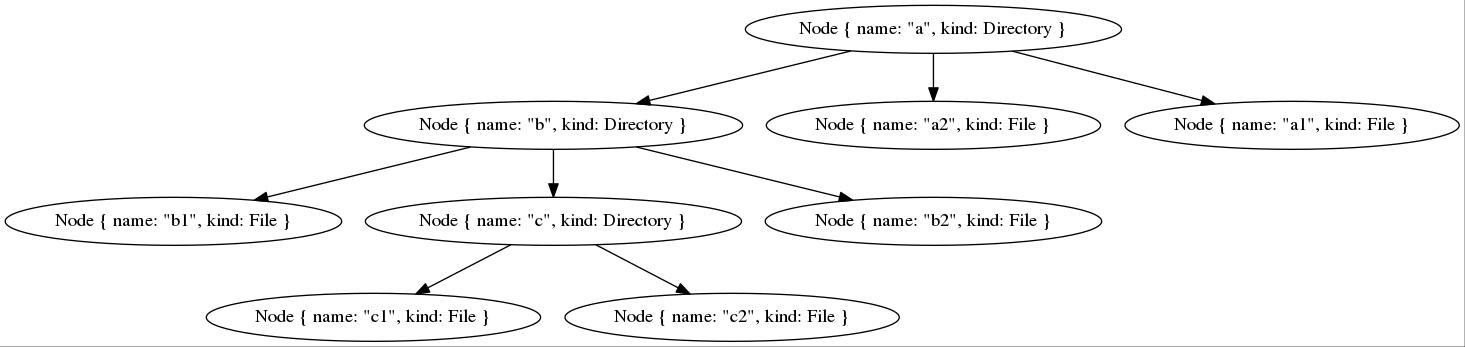
\includegraphics[width=1\textwidth]{images/graph.jpg}
    \end{center}
    \caption{légende}
    \label{label}
\end{figure}